\documentclass{sig-alternate}
\usepackage[numbers, sort, compress]{natbib}
\usepackage{graphics}
\usepackage{graphicx}
\usepackage{epstopdf}
\usepackage{color}
\usepackage{hyperref}
\usepackage{pdfsync}
\usepackage{mdwlist}


\begin{document}

\conferenceinfo{} {}
\CopyrightYear{2011}
\crdata{}
%\clubpenalty=10000
%\widowpenalty = 10000


\title{Computational Characteristics of Data-Intensive Computing with NGS Short-read Aligners : Distributed Computing Perspective}

\numberofauthors{6}
\author{
\alignauthor Joohyun Kim\titlenote{Author for correspondence, e-mail : jhkim@cct.lsu.edu}\\
       \affaddr{Center for Computation and Technology}\\
       \affaddr{Louisiana State University}\\
       \affaddr{216 Johnston}\\
       \affaddr{Baton Rouge, LA} \\
  %     \email{jhkim@cct.lsu.edu}
\alignauthor Sharath Maddineni\\
       \affaddr{Center for Computation and Technology}\\
       \affaddr{Louisiana State University}\\
       \affaddr{216 Johnston}\\
       \affaddr{Baton Rouge, LA}
   %    \email{smaddineni@cct.lsu.edu}
\alignauthor Mark Santcroos\\
       \affaddr{Center for Computation and Technology}\\
       \affaddr{Louisiana State University}\\
       \affaddr{216 Johnston}\\
       \affaddr{Baton Rouge, LA}
  %     \email{}
       \and
\alignauthor Ole Weidner\\
       \affaddr{Center for Computation and Technology}\\
       \affaddr{Louisiana State University}\\
       \affaddr{216 Johnston}\\
       \affaddr{Baton Rouge, LA}
%       \email{oweinder@cct.lsu.edu}
\alignauthor Shantenu Jha\titlenote{Author for correspondence, e-mail : sjha@cct.lsu.edu}\\
      \affaddr{Center for Computation and Technology}\\
     \affaddr{Louisiana State University}\\
      \affaddr{214 Johnston}\\
      \affaddr{Baton Rouge, LA}
%     \email{sjha@cct.lsu.edu}
}

\maketitle



\begin{abstract}
We present the survey of Short-read Aligners of Next-Generation DNA Sequencing Data.  Our interest is, in particular, to understand their computational requirements and characteristic aspects with respect to their capacity as distributed applications.  
  
  
\end{abstract}

\newif\ifdraft
%\drafttrue                                                                                        \
\ifdraft
% \newcommand{\reviewer}[1]{ {\textcolor{blue}    { ***Reviewer:     #1 }}}
 \newcommand{\jkimnote}[1]{{\textcolor{green}   { ***Joohyun:   #1 }}}
 \newcommand{\jhanote}[1]{  {\textcolor{red}     { ***SJ: #1 }}}
  \newcommand{\smnote}[1]{  {\textcolor{red}     { ***Sharath: #1 }}}
 \newcommand{\todo}[1]{  {\textcolor{red}     { ***TODO: #1 }}}
 \newcommand{\fix}[1]{  {\textcolor{red}     { ***FIX: #1 }}}
 \newcommand{\reviewer}[1]{}
\else
 \newcommand{\reviewer}[1]{}
 \newcommand{\jkimnote}[1]{}
 \newcommand{\smnote}[1]{}
 \newcommand{\jhanote}[1]{}
 \newcommand{\todo}[1]{  {\textcolor{red}     { ***TODO: #1 }}}
 \newcommand{\fix}[1]{}                                                                              
 \fi



\category{D.1.3}{Software}{Concurrent Programming}{ Distributed programming/parallel programming} 
\category{J.3}{Computer Applications}{Bioinformatics}

  
\section*{General Terms}{Design,Measurement,Theory}

 \keywords{Short-read Aligner, Distributed Computing, Simple API for Grid
  Applications (SAGA), Pilot-Job abstraction, Data-intensive Computing}

\section{INTRODUCTION}

%\begin{figure}
% \centering
%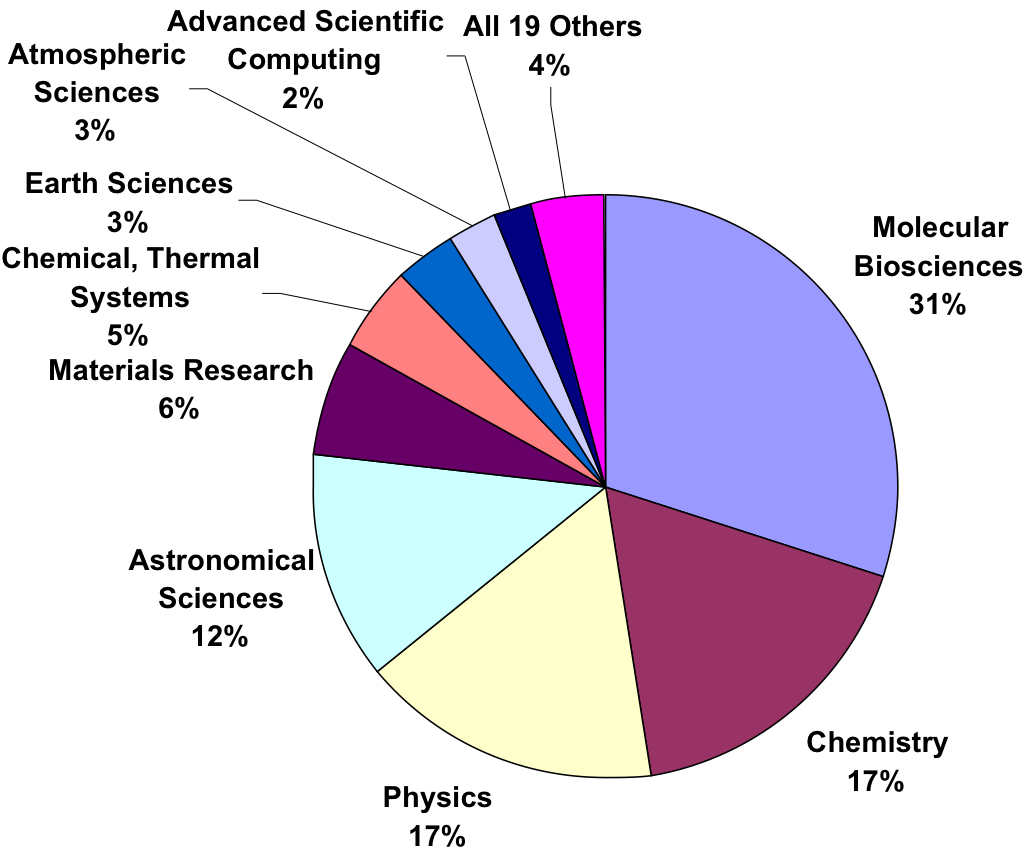
\includegraphics[scale=0.40]{figures/teragrid-discipline07}
%\caption{\small 2007 Usage statistics for the TeraGrid.  (Reference
%  \url{http://www.teragridforum.org/mediawiki/images/9/90/II_WorkShop_G-HPC_Nework_2009-Towns.pdf})}
%  \label{tg2007}
%\end{figure}


\begin{table}
 \small
\begin{tabular}{|c|c|c|c|c|c|} 
  \hline  Name & BFAST  & BWA & Novoalign & SHRiMP2  & SOAP2  \\ 
\hline \hline

Ref. Genome  & & & & & \\
Indexing & & & & & \\ \hline
Alignment & & & & & \\
 & & & & & \\ \hline
Color Space  & Yes & Yes & Yes & Yes & No\\ \hline
\textbf{Fine-grain} &  &  &  &  & \\ 
 \textbf{Parallelism} & & & & & \\
Multi-threading & Yes & & Yes & Yes & \\ 
MPI & & & Yes & & \\
OpenMP &  & &  & Yes & \\  \hline
\textbf{Coarse-grain}  & & & & & \\ 
\textbf{Paralleism} & & & & & \\
& & & & & \\ \hline
\end{tabular} 
\caption{Overall comparison of the mapping tools surveyed in this work.}
 \label{global-comp} 
\end{table}


\section{Algorithmic Characteristics}
\textit{Reference genome indexing}



\textit{Alignment candidate finding}


\textit{Local alignment}



\section{Computational Requirement}
\textit{Fine-grain parallelism support}



\textit{Reference index management}


\textit{Task level concurrency support}






\begin{table}

\begin{tabular}{|c|c|c|c|}  \hline
  & Memory & Disk-space &  \\  \hline 
Indexing  & 16 GB & 130 GB &  \\
  & & &  \\ 
 & & &  \\
 & & &  \\ \hline

\end{tabular} 
\caption{Computational requirement for BFAST with hg18 as a reference genome.  hg18 is composed of 2.7 GB}
 \label{comp-req-bfast} 
\end{table}

\begin{table}
\begin{tabular}{|c|c|c|c|}  \hline
  & Memory & Disk-space &  \\  \hline 
Indexing  & &  &  \\
  & & &  \\ 
 & & &  \\
 & & &  \\ \hline

\end{tabular} 
\caption{Computational requirement for BWA with hg18 as a reference genome.  hg18 is composed of 2.7 GB}
 \label{comp-req-bwa} 
\end{table}

\begin{table}

\begin{tabular}{|c|c|c|c|}  \hline
  & Memory & Disk-space &  \\  \hline 
Indexing  & 48 GB (+ 0.75 GB + 0.05 GB) & &  \\
  & & &  \\ 
 & & &  \\
 & & &  \\ \hline

\end{tabular} 
\caption{Computational requirement for SHRiMP with hg18 as a reference genome.  hg18 is composed of 2.7 GB}
 \label{comp-req-shrimp} 
\end{table}

\begin{table}

\begin{tabular}{|c|c|c|c|}  \hline
  & Memory & Disk-space &  \\  \hline 
Indexing  &   & 8 GB &  \\
  & & &  \\ 
 & & &  \\
 & & &  \\ \hline

\end{tabular} 
\caption{Computational requirement for NovoalignCS with hg18 as a reference genome.  hg18 is composed of 2.7 GB}
 \label{comp-req-novoCS} 
\end{table}



\section{Dat-intensive Computing as a Distributed Application}


\section{Conclusions}



\section{Acknowledgments}
We are grateful to Andre Luckow for his work for SAGA-BigJob development.  Computing resources used for this
work were made possible via NSF TRAC award TG-MCB090174 and LONI
resources.  This document was developed with support from the National
Science Foundation (NSF) under Grant No.  0910812 to Indiana
University for ``FutureGrid: An Experimental, High-Performance Grid
Test-bed.'' The project described was partially supported by Grant
Number P20RR016456 from the NIH National Center For Research
Resources. SJ would like to thank Dave Hart (SDSC) and Dan Katz
(Chicago) for helpful discussions.

\bibliographystyle{abbrv}
\bibliography{}
\end{document}



% \textit{Achieving IDEAS : Interoperability, Distributed
%   scaled-out, Extensibility, Adaptivity, and Simplicity}

%\smnote{ 1) Lets say we have "n" read files and with DARE it takes
%  around time "t" time for matching step if we run it serially it
%  would take n*t time. It probably exceeds wall time limit. Therefore
%  speed up in match step depends how many number of read files we
%  generate and process concurrently.  2) Yes we were able to process
%  the complete run with entire Human Genome on QB and Ranger
%  separately. (**I am currently working this to utilizing QB and
%  Ranger together.)  4) it should clearly provide the advantage with
%  multiple resources. If we want to use the cloud resources from India
%  to complete Human Genome run it is not practically possible because
%  of the current limited disk size access provided by the FG
%  Eucalyptus resources. Because whole human genome index files are of
%  size 129 GB for Bfast matching step as opposed to HG 18 Chromosome
%  21 with size of 2 GB index files. On the other hand it also requires
%  the temporary files disk space.  Thus it is important to utilize
%  large capacity resources like QB and Ranger divide the work load
%  across machines.}  
  
%   Here, we present how the objectives of IDEAS\cite{ideas} are
% accomplished with the DARE gateway examples. 
